\en

\section**{Problem outline}
\label{sec:problem}

The Linux kernel is a Free/Libre/Open-Source project providing value to
billions of people daily, representing 96.3\% of the top one million web
servers and 85\% of smartphones worldwide. The magnitude that the project has
reached over the years makes the addition of features, as well as handling bugs
and security vulnerabilities, potentially affect a significant number of
people, demonstrating the importance of maintaining the kernel
\citep{linuxdata}.

Maintaining the Linux kernel is a complex task, as the project contains more
than 19 million lines of code and has had over thirteen thousand contributors
throughout its lifespan \citep{linuxquantity}. Given the magnitude of the Linux
kernel project, it is unrealistic to expect that all contributors have
consistently followed the best programming practices and principles in every
contribution made to the project. Consequently, it is expected that a
significant amount of low-quality code artifacts will be found in the source
code, which could hinder or compromise the maintenance of the project and the
addition of new features.

As stated by \citet{driverdef}, device drivers are a ``piece of software whose
aim is to control and manage a particular hardware device, hence the name
device driver.'' Device drivers are a major part of the Linux kernel,
representing 66\% of the source code, and are responsible for managing
essential elements such as keyboards, mice, and GPUs \citep{marcelo}. When the
kernel opts to support new hardware, it necessitates alterations to existing
device drivers or the creation of new ones, making maintaining device drivers a
critical duty of the Linux community.

The AMD Display driver in the Linux kernel is responsible for enabling AMD GPUs
to operate correctly in desktop Linux environments, which is an essential task,
given that AMD GPUs represented 19\% of the personal GPU market in 2023
\citep{gpumarket}. When we interacted with the maintainers of the AMD Display
driver, they shared with us their challenges regarding one of the
characteristics of low-quality code artifacts: duplicated code, which hampers
the maintenance of the driver.

In searching for solutions to the AMD Display driver problem related to
duplicated code artifacts, we found tools capable of determining, given two
code artifacts, whether they are duplications of each other. However, the
formal literature on code duplication mainly focuses on optimizing the accuracy
of these tools for this specific task. These solutions do not address our
problem, as we cannot provide a complete codebase and have the tools return the
code duplications within it. Moreover, they do not guide us on how to mitigate
the code duplications after detection, necessitating the exploration of
alternative solutions.

Given the unsuccessful results of our search in the formal literature, we
turned to gray literature for solutions but were also met with limited success.
The best solutions we found in the gray literature were primitive, merely
identifying every pair of code files that are duplications. The code files in
the AMD Display driver containing duplicated code typically have specific code
unique to each file. Therefore, a solution that identifies duplication in a
deeper context is necessary to find accurate duplications within the Linux
kernel context.


\section**{Research Design}

According to our studies and observations, the code duplication problem
outlined in the section above cannot be resolved by the solutions presented in
the formal or gray literature. To address this gap, we propose an approach to
identify and mitigate code duplications in the Linux kernel. Specifically, we
aim to develop a tool capable of detecting duplicated functions within the
kernel and establish strategies for mitigating these duplications.

In this research, we expect to extract patterns of software engineering
techniques, such as refactoring methods commonly used to mitigate code
duplications. These patterns will guide future contributors in tackling the
code duplication problem in the given context. To properly investigate our
proposed approach, we developed the following primary research question to
guide our study:

\textbf{RQ1:} What are effective approaches for identifying duplicate code in the
Linux kernel?

Given the complexity of the primary question, we formulated a supplementary
research question to assess midway results related to the performance of our
proposed tool in the Linux kernel. The supplementary research question is
defined as follows:

\textbf{RQ1.1:} How accurately does an approach detect duplicated functions
within the Linux kernel?

We adopt a multi-method research design utilizing various methodologies
throughout the study to address our research questions. We structured this work
into two phases, each employing distinct research methods.

In \textbf{Phase I}, we will propose, develop, and validate a tool capable of
identifying code duplications at the function level for the C programming
language. We expect this tool to effectively identify code duplications in the
Linux kernel, as our preliminary investigation suggests that code files in the
kernel often contain a mix of duplicated and non-duplicated functions. To
validate the tool, we will perform a triangulation of results by evaluating our
tool against code duplication databases used in the formal literature and by
conducting an empirical analysis on a randomly selected set of code files from
the AMD Display driver, which our tool identifies as containing duplications.
Chapter \ref{cha:method} provides a detailed explanation of our validation
process.

\begin{figure}[h]
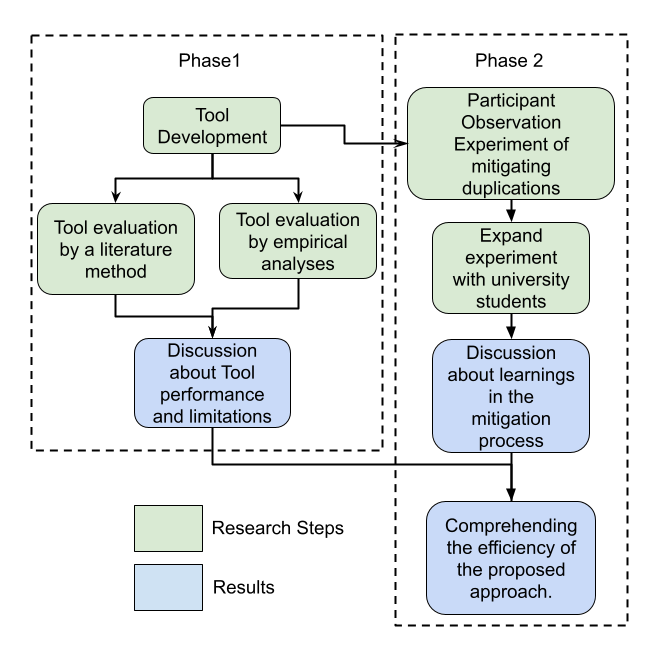
\includegraphics[scale=0.7]{research_design}
\caption{Diagram of the research design.}
\label{fig:reDesign}
\end{figure}

Upon completing the first phase, we will have a validated tool for identifying
code duplications within the Linux kernel context. We can then proceed to the
second phase of our research, which focuses on mitigating these duplications.
In \textbf{Phase II}, we aim to discover practical strategies to address the
code duplications detected in the Linux kernel. To achieve this objective, we
have designed an ethnographic approach that allows us to interact with the
Linux community and collect artifacts that validate or refute our proposed
mitigation strategies.

Figure \ref{fig:reDesign} summarizes the research steps proposed in this work.

\section**{Manuscript Structure}


This manuscript consists of five more chapters. Chapter \ref{cha:back} presents
the literature overview for code duplication detection (main definitions,
current approaches in the literature), a brief description of the Linux kernel,
and a review of refactoring methods used throughout this research. Chapter
\ref{cha:tool} presents our proposed tool to detect code duplication in the
Linux kernel, describing all the main components.  Chapter \ref{cha:method}
describes the research methods selected to guide our work. Chapter
\ref{cha:eval} shows the results obtained from the research methods to evaluate
our proposed tool. Chapter \ref{cha:results} presents the current research
stage and the work plan, with the addition of preliminary results obtained.
